% !TEX encoding = UTF-8 Unicode
% !TEX spellcheck = en-US

\documentclass[10pt,a4paper,titlepage]{article}
\usepackage[utf8]{inputenc}
\usepackage[T1]{fontenc}
\usepackage{amsmath}
\usepackage{ragged2e}
\usepackage{hyperref}
\usepackage{amsfonts}
\usepackage{amssymb}
\usepackage{graphicx}
\usepackage{xcolor}
\usepackage{listings}
\usepackage{minted}
\hypersetup{
	colorlinks=true,
	linkcolor=blue,
	filecolor=magenta,      
	urlcolor=cyan,
}
\definecolor{codegreen}{rgb}{0,0.6,0}
\definecolor{codegray}{rgb}{0.5,0.5,0.5}
\definecolor{codepurple}{rgb}{0.58,0,0.82}
\definecolor{backcolour}{rgb}{0.95,0.95,0.92}

\lstdefinestyle{mystyle}{
	backgroundcolor=\color{backcolour},   
	commentstyle=\color{codegreen},
	keywordstyle=\color{magenta},
	numberstyle=\tiny\color{codegray},
	stringstyle=\color{codepurple},
	basicstyle=\ttfamily\footnotesize,
	breakatwhitespace=false,         
	breaklines=true,                 
	captionpos=b,                    
	keepspaces=true,                 
	numbers=left,                    
	numbersep=5pt,                  
	showspaces=false,                
	showstringspaces=false,
	showtabs=false,                  
	tabsize=2
}

\lstset{style=mystyle}

\urlstyle{same}
\author{Yapi D}
\title{Lab 2}


\begin{document}
	\makeatletter
\begin{titlepage}
	\begin{center}
		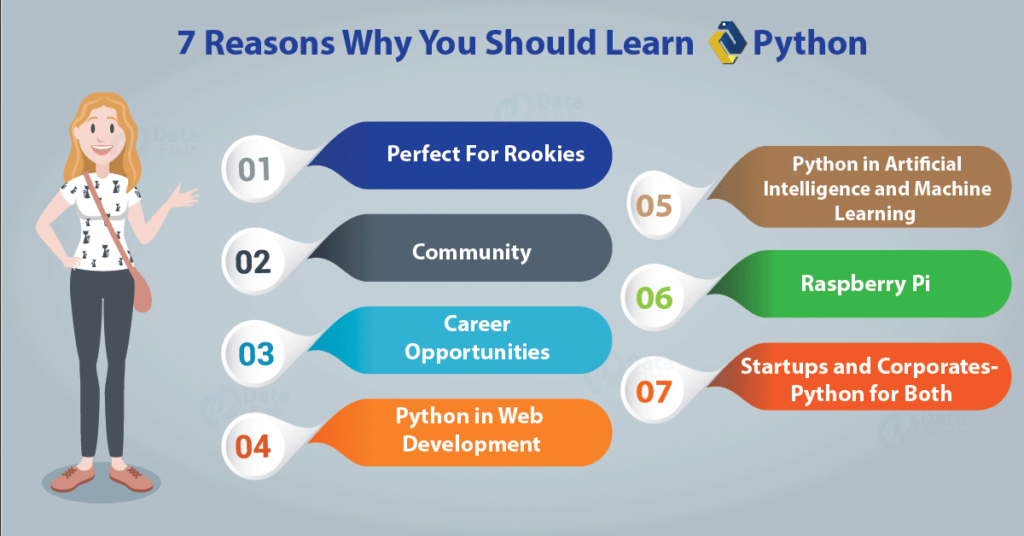
\includegraphics[width=1\linewidth]{pylogo}\\[4ex]
		{\huge \bfseries  \@title }\\[2ex] 
		{\LARGE  \@author}\\[50ex] 
		{\large \@date}
	\end{center}
\end{titlepage}
\makeatother
\thispagestyle{empty}
\newpage

	




\section{Function and string}
In this lab you will learn about functions that take arguments and return something. \textcolor{blue}{I encourage you to bring an extra bigger screen. It will make programming easier for you in this lab}.
\justify
You will learn how to import your function in an other python file. You will write two functions: the first function will take a table as argument and return two parameters (frequency and amplitude data).
\justify
 The second function will return two strings representing the x label and the y label for a plot. Then you will import both functions into a dashboard program. We will be using the python dashboard library called dash. So we need to install it.
The user will upload a file into the dashboard and the dashboard should show the plot as bellow 
\begin{figure}[H]
	\centering
	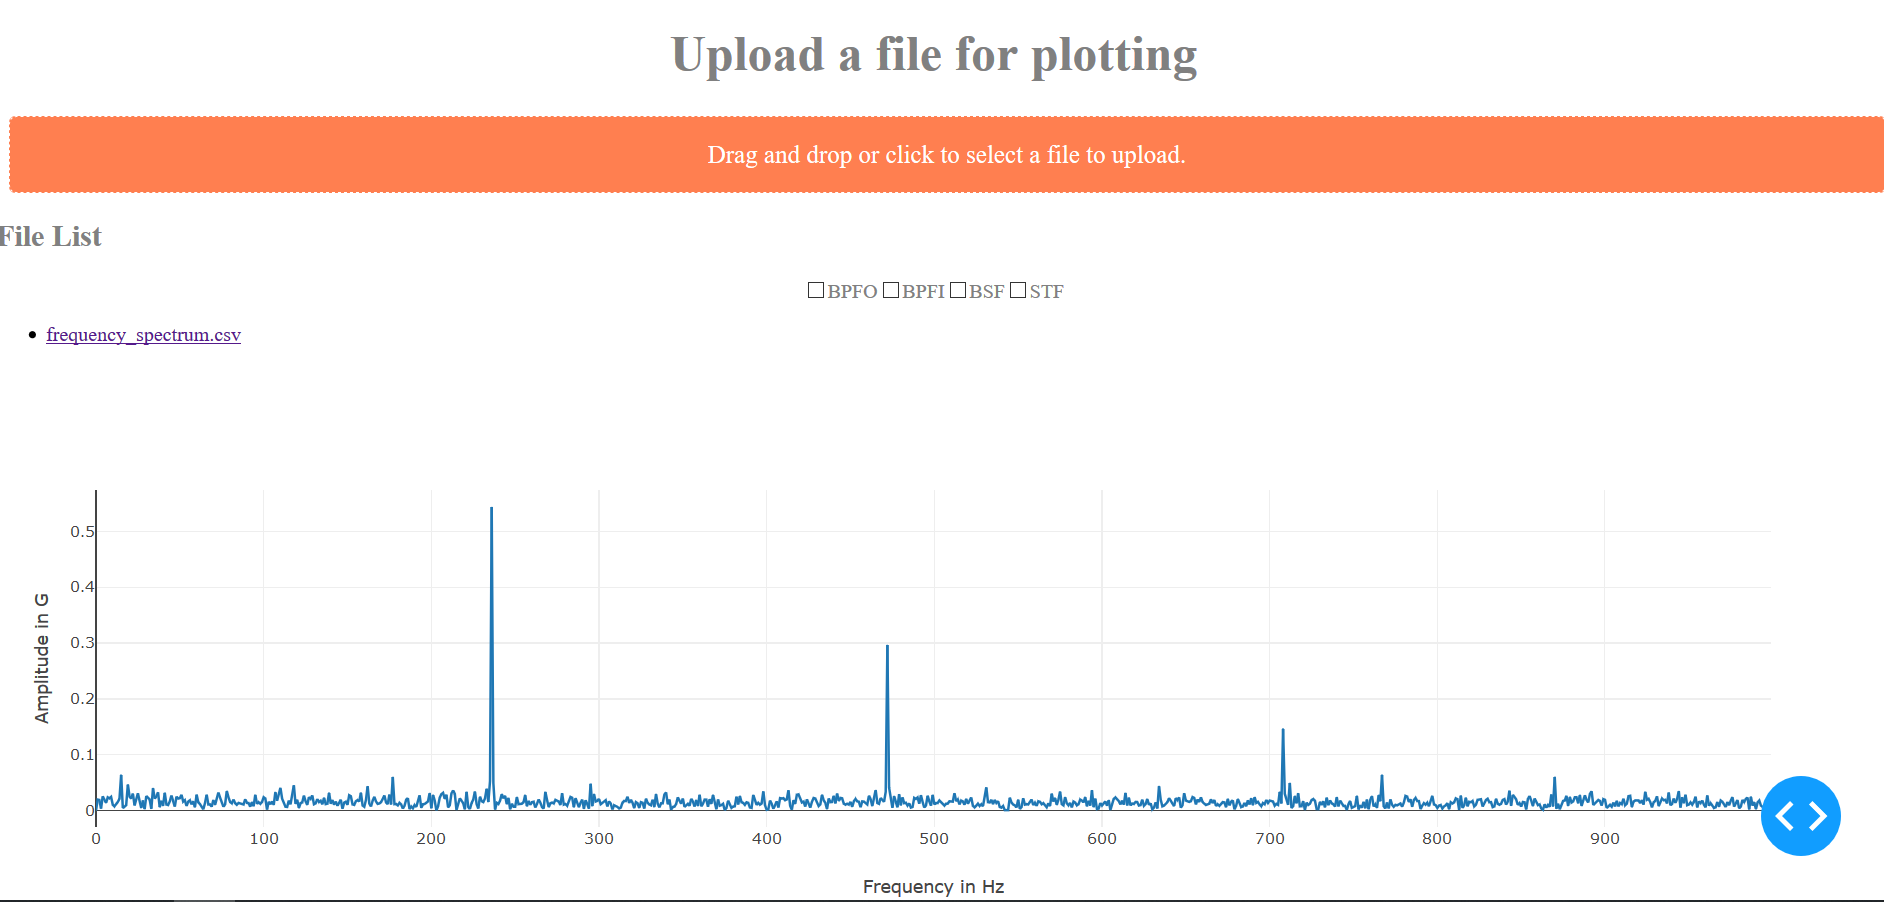
\includegraphics[width=1.5\linewidth]{dashboard}
\end{figure}
\justify
 
\subsection{First push the code of lab 1 on github} 
You start this lab by pushing the code you wrote on lab 1 on github.

\begin{lstlisting}[language=python]
#add all your code on git
$ git add -A

#tell git that you are sure about adding the files
$ git commit -m "I am adding my code bla bla bla"

#push your code on the git server
 $ git push
\end{lstlisting}

\subsection{Create a virtual environment and install packages}
\begin{lstlisting}[language=python]
# create a virtual environment called lab2-env
$ python -m venv lab2-env

# if you get an error copy past this scrit
$ Set-ExecutionPolicy Unrestricted -Scope CurrentUser

# activate your virtual environement
$ lab2-env\Scripts\activate

# go inside you workiing directory
$ cd path\to\working\directory

# create a file called requirements
$ New-Item requirement.txt

# install some packages
$ pip install numpy
$ pip install pandas
$ pip install dash
$ pip install flask
$ pip install plotly
$ pip install dash_core_components
$ pip install dash_html_components

\end{lstlisting}
\subsection{Function returning something, and list}
So far we have seen functions that print something. Now we will write functions that return something
\begin{lstlisting}[language=python]
# a funtion that returns a string
def get_name():
	name = "Yapi"
	return name
	
# now call the function and print
name = get_name()
print(name)
\end{lstlisting}

\begin{lstlisting}[language=python]
# a funtion that returns two strings
def get_name_and_job():
name = "Yapi"
job = "Astronaut"
return name, job

# now call the function and print
name, job = get_name_and_job()
print(name, job)
message = "{} is an {}".format(name, job)
print(message)
\end{lstlisting}
Today we will learn about  python list. A list is a collection of items in a square bracket:
\begin{lstlisting}[language=python]
# alist of number
my_list = [1,2,3,4,4]
# a list of strings
my_strings_list = ["bla", "blabla", "cool", "yes"]
\end{lstlisting}
the place of each item in a list is called \textcolor{blue}{index}. for example "bla" is at index 0, "blabla" is at index 1, "cool" is at index 2 and "yes" is at index 3. You can access an item of a list by specifying its index like this :
\begin{lstlisting}[language=python]
my_strings_list[0], my_strings_list[1]
\end{lstlisting}
One import function to split list in python is the function called split()
\begin{lstlisting}[language=python]
def split_list(string):
	"""
	This function take a a string 
	as argument, split it and return 
	a list of substrings.
	"""
	strings_list = string.split()
	return strings_list

# call the function and print:
string = "What is happening here guys"
string_list = split_list(string)
print(string_list)
print(string_list[0])
print(string_list[1])
print(string_list[-1])
\end{lstlisting}

\begin{lstlisting}[language=python]
def split_list2(string):
"""
This function take a a string 
as argument, split it and return 
a list of substrings.
"""
strings_list = string.split("/")
return strings_list

# call the function and print:
string = "What/is/happening/here/guys"
string_list = split_list(string)
print(string_list)
print(string_list[0])
print(string_list[1])
print(string_list[-1])
\end{lstlisting}
\subsection{Exercise}
Write a function that return the strings "Amplitude in G" and "Frequency in Hz"
\subsection{Exercise}
write a function that takes a table as argument and return frequency and amplitude data.
use the functions you wrote in lab1.

\section{Import function in an other python file}
\begin{enumerate}
	\item In your working directory, create a file called get$\_$data.py
	\begin{lstlisting}
	$ New-item get_data.py
	\end{lstlisting}
	\item in powershell run the file dashboard.py
\begin{lstlisting}
$ python dashboard.py
copy http://127.0.0.1:8888/ and past it in your browser
\end{lstlisting}

\item copy and past the two functions that you created in exercise 1.4 and 1.5 in the file get$\_$data.py
dont forget to import pandas.
\item go to the file dashboard.py and at the top import the two functions from the file get$\_$data.py
\begin{lstlisting}
$ from get_data import function_number1, function_number2
\end{lstlisting}
\item go in the file dashboad.py scroll down until you see : This is the function you need to update.
Call your functions, and go to the dashboard to upload your file (the one we used last time)
Now you should see a plot of the frequency spectrum in the dashboard.
\end{enumerate}



\end{document}